\documentclass[12pt, a4paper, english, singlespacing, parskip]{scrartcl}

%\documentclass[
%11pt, 				% The default document font size, options: 10pt, 11pt, 12pt
%oneside, 			% Two side (alternating margins) for binding by default, uncomment to switch to one side
%chapterinoneline,	% Have the chapter title next to the number in one single line
%english, 			% ngerman for German
%singlespacing, 	% Single line spacing, alternatives: onehalfspacing or doublespacing
%draft, 			% Uncomment to enable draft mode (no pictures, no links, overfull hboxes indicated)
%nolistspacing, 	% If the document is onehalfspacing or doublespacing, uncomment this to set spacing in lists to single
%liststotoc, 		% Uncomment to add the list of figures/tables/etc to the table of contents
%toctotoc, 			% Uncomment to add the main table of contents to the table of contents
%parskip, 			% Uncomment to add space between paragraphs
%nohyperref, 		% Uncomment to not load the hyperref package
%headsepline, 		% Uncomment to get a line under the header
%]{scrartcl or scrreprt or scrbook} % The class file specifying the document structure

\usepackage{amssymb, amsmath, color, graphicx, float, setspace, tipa}
\usepackage[utf8]{inputenc} 
\usepackage[english]{babel}
\usepackage[pdfpagelabels,pdfstartview = FitH,bookmarksopen = true,bookmarksnumbered = true,linkcolor = black,plainpages = false,hypertexnames = false,citecolor = black, breaklinks]{hyperref}
\usepackage{url}
\usepackage{caption}
\captionsetup{font=small,labelfont=bf, format=plain, justification=centering}
\allowdisplaybreaks 		% allows page breaks in align/equation environment

\usepackage{authblk} 		% titlepage stuff
\usepackage[titletoc, title]{appendix}



%--------------------------------------------
% NEW COMMANDS
%--------------------------------------------

\newcommand{\corresponds}{\mathrel{\widehat{=}}}		% equals with hat

\newcommand {\arctanh}{\mathrm{arctanh}}				% Atanh
\newcommand{\arccot}{\mathrm{arccot }}					% Acotanh

\newcommand{\limz}[1]{\lim\limits_{#1 \rightarrow 0}}	% Limes of something towars zero

\newcommand{\bm}{\boldmath}								% Bold font in math
\newcommand{\dps}{\displaystyle}						

\newcommand{\e}{\mbox{e}}								% e noncursive in math mode

\newcommand{\del}{\partial}								% partial diff operator
\newcommand{\de}{\mathrm{d}}							% differential d
\newcommand{\D}{\mathrm{d}}								% differential d
\newcommand{\GRAD}{\mathrm{grad}\ }						% gradient
\newcommand{\DIV}{\mathrm{div}\ }						% divergence
\newcommand{\ROT}{\mathrm{rot}\ }						% rotation

\newcommand{\CONST}{\mathrm{const.\ }}					% constant
\newcommand{\var}{\mathrm{var}}							% variance

\newcommand{\g}{^\circ}									% degrees
\newcommand{\degr}{^\circ}								% degrees

\newcommand{\msol}{M_\odot}								% solar mass


\newcommand{\x}{\mathbf{x}}								% x vector
\newcommand{\xdot}{\dot{\mathbf{x}}}					% x dot vector
\newcommand{\xddot}{\ddot{\mathbf{x}}}					% x doubledot vector
\newcommand{\R}{\mathbf{r}}								% r vector
\newcommand{\rdot}{\dot{\mathbf{r}}}					% r dot vector
\newcommand{\rddot}{\ddot{\mathbf{r}}}					% r doubledot vector
\newcommand{\vel}{\mathbf{v}}							% v vector
\newcommand{\V}{\mathbf{v}}								% v vector
\newcommand{\vdot}{\dot{\mathbf{v}}}					% v dot vector
\newcommand{\vddot}{\ddot{\mathbf{v}}}					% v doubledot vector

\newcommand{\dete}{\mathrm{d}t}							% dt
\newcommand{\delte}{\del t}								% partial t
\newcommand{\dex}{\mathrm{d}x}							% dx
\newcommand{\delx}{\del x}								% partial x
\newcommand{\der}{\mathrm{d}r}							% dr
\newcommand{\delr}{\del r}								% partial r

\newcommand{\deldt}{\frac{\del}{\del t}}				% shortcut partial derivative, in line
\newcommand{\ddt}{\frac{\de}{\de t}}					% shortcut total derivative, in line
\newcommand{\DELDT}[1]{\frac{\del  #1}{\del t}}			% shortcut partial derivative, on fraction
\newcommand{\DDT}[1]{\frac{\de  #1}{\de t}}				% shortcut total derivative, on fraction

\newcommand{\deldx}{\frac{\del}{\del x}}				% shortcut partial derivative, in line
\newcommand{\ddx}{\frac{\de}{\de x}}					% shortcut total derivative, in line
\newcommand{\DELDX}[1]{\frac{\del  #1}{\del x}}			% shortcut partial derivative, on fraction
\newcommand{\DDX}[1]{\frac{\de  #1}{\de x}}				% shortcut total derivative, on fraction

\newcommand{\deldr}{\frac{\del}{\del r}}				% shortcut partial derivative, in line
\newcommand{\ddr}{\frac{\de}{\de r}}					% shortcut total derivative, in line
\newcommand{\DELDR}[1]{\frac{\del  #1}{\del r}}			% shortcut partial derivative, on fraction
\newcommand{\DDR}[1]{\frac{\de  #1}{\de r}}				% shortcut total derivative, on fraction


\newcommand{\U}{\mathbf{U}}                             % state vector
\newcommand{\F}{\mathbf{F}}                             % flux tensor
\newcommand{\half}{\tfrac{1}{2}}

% quickly insert a figure without a caption
% usage: \quickfig{filename}{label}
\newcommand{\quickfig}[2]{
	\begin{figure}[H]
		\includegraphics[width=\textwidth]{#1}
		\caption{\label{#2}}
	\end{figure}
}


% replace \sum with \sum\limits
\let\oldsum\sum
\renewcommand{\sum}{\oldsum\limits}




%-----------------------------------------------
% FORMAT TITLE
%-----------------------------------------------


% Set fonts of document parts
\setkomafont{title}{\rmfamily\bfseries\boldmath}
\addtokomafont{section}{\rmfamily\bfseries\boldmath}
\addtokomafont{subsection}{\rmfamily\bfseries\boldmath}
\addtokomafont{subsubsection}{\rmfamily\bfseries\boldmath}
\addtokomafont{disposition}{\rmfamily} % table of contents and stuff
\setkomafont{descriptionlabel}{\rmfamily\bfseries\boldmath}




%------------------------------------------
%: Metadata
%------------------------------------------

\title{Test Results for Mesh Hydro Code}
\author{This computer}
\date{}

%------------------------------------------








\begin{document}
	

%Titlepage
\maketitle

\tableofcontents
\clearpage



\section{Advection}

\subsection{Piecewise Constant}

\begin{figure}[htbp]
    \centering
	\includegraphics[width=.7\textwidth]{./figures/advection-1D-pwconst-density-only-overplotted.png}%
	\caption{Expected result 1D}
	\includegraphics[width=.7\textwidth]{../advection-1D-pwconst-density-only-overplotted.png}%
	\caption{Obtained result 1D}
\end{figure}

\begin{figure}[htbp]
    \centering
	\includegraphics[width=.7\textwidth]{./figures/advection-1D-pwconst-negvel-density-only-overplotted.png}%
	\caption{Expected result 1D negative velocity}
	\includegraphics[width=.7\textwidth]{../advection-1D-pwconst-negvel-density-only-overplotted.png}%
	\caption{Obtained result 1D negative velocity}
\end{figure}

\begin{figure}[htbp]
    \centering
	\includegraphics[width=.7\textwidth]{./figures/advection-2D-pwconst-0001-density-only.png}%
	\caption{Expected result 2D}
	\includegraphics[width=.7\textwidth]{../advection-2D-pwconst-0001-density-only.png}%
	\caption{Obtained result 2D}
\end{figure}

\begin{figure}[htbp]
    \centering
	\includegraphics[width=.7\textwidth]{./figures/advection-2D-pwconst-negvel-0001-density-only.png}%
	\caption{Expected result 2D negative velocity}
	\includegraphics[width=.7\textwidth]{../advection-2D-pwconst-negvel-0001-density-only.png}%
	\caption{Obtained result 2D negative velocity}
\end{figure}

\begin{figure}[htbp]
    \centering
	\includegraphics[width=.7\textwidth]{./figures/advection-2D-pwconst-x-0001-density-only.png}%
	\caption{Expected result 2D velocity in x direction only}
	\includegraphics[width=.7\textwidth]{../advection-2D-pwconst-x-0001-density-only.png}%
	\caption{Obtained result 2D velocity in x direction only}
\end{figure}

\begin{figure}[htbp]
    \centering
	\includegraphics[width=.7\textwidth]{./figures/advection-2D-pwconst-y-0001-density-only.png}%
	\caption{Expected result 2D velocity in y direction only}
	\includegraphics[width=.7\textwidth]{../advection-2D-pwconst-y-0001-density-only.png}%
	\caption{Obtained result 2D velocity in y direction only}
\end{figure}






\clearpage
\subsection{Piecewise Linear}

\begin{figure}[htbp]
    \centering
	\includegraphics[width=.7\textwidth]{./figures/advection-1D-pwlin-density-only-overplotted.png}%
	\caption{Expected result 1D}
	\includegraphics[width=.7\textwidth]{../advection-1D-pwlin-density-only-overplotted.png}%
	\caption{Obtained result 1D}
\end{figure}

\begin{figure}[htbp]
    \centering
	\includegraphics[width=.7\textwidth]{./figures/advection-1D-pwlin-negvel-density-only-overplotted.png}%
	\caption{Expected result 1D negative velocity}
	\includegraphics[width=.7\textwidth]{../advection-1D-pwlin-negvel-density-only-overplotted.png}%
	\caption{Obtained result 1D negative velocity}
\end{figure}

\begin{figure}[htbp]
    \centering
	\includegraphics[width=.7\textwidth]{./figures/advection-2D-pwlin-0001-density-only.png}%
	\caption{Expected result 2D}
	\includegraphics[width=.7\textwidth]{../advection-2D-pwlin-0001-density-only.png}%
	\caption{Obtained result 2D}
\end{figure}

\begin{figure}[htbp]
    \centering
	\includegraphics[width=.7\textwidth]{./figures/advection-2D-pwlin-negvel-0001-density-only.png}%
	\caption{Expected result 2D negative velocity}
	\includegraphics[width=.7\textwidth]{../advection-2D-pwlin-negvel-0001-density-only.png}%
	\caption{Obtained result 2D negative velocity}
\end{figure}

\begin{figure}[htbp]
    \centering
	\includegraphics[width=.7\textwidth]{./figures/advection-2D-pwlin-x-0001-density-only.png}%
	\caption{Expected result 2D velocity in x direction only}
	\includegraphics[width=.7\textwidth]{../advection-2D-pwlin-x-0001-density-only.png}%
	\caption{Obtained result 2D velocity in x direction only}
\end{figure}

\begin{figure}[htbp]
    \centering
	\includegraphics[width=.7\textwidth]{./figures/advection-2D-pwlin-y-0001-density-only.png}%
	\caption{Expected result 2D velocity in y direction only}
	\includegraphics[width=.7\textwidth]{../advection-2D-pwlin-y-0001-density-only.png}%
	\caption{Obtained result 2D velocity in y direction only}
\end{figure}








\clearpage
\subsection{Piecewise Linear with Slope Limiters}

\begin{figure}[htbp]
    \centering
	\includegraphics[width=.7\textwidth]{./figures/advection-1D-MINMOD-density-only-overplotted.png}%
	\caption{Minmod Slope Limiter. Expected result 1D}
	\includegraphics[width=.7\textwidth]{../advection-1D-MINMOD-density-only-overplotted.png}%
	\caption{Minmod Slope Limiter. Obtained result 1D}
\end{figure}

\begin{figure}[htbp]
    \centering
	\includegraphics[width=.7\textwidth]{./figures/advection-1D-SUPERBEE-density-only-overplotted.png}%
	\caption{Superbee slope limiter. Expected result 1D negative velocity}
	\includegraphics[width=.7\textwidth]{../advection-1D-SUPERBEE-density-only-overplotted.png}%
	\caption{Superbee slope limiter. Obtained result 1D negative velocity}
\end{figure}

\begin{figure}[htbp]
    \centering
	\includegraphics[width=.7\textwidth]{./figures/advection-1D-MC-density-only-overplotted.png}%
	\caption{Monotonized central limiter. Expected result 1D}
	\includegraphics[width=.7\textwidth]{../advection-1D-MC-density-only-overplotted.png}%
	\caption{Monotonized central limiter. Obtained result 1D}
\end{figure}

\begin{figure}[htbp]
    \centering
	\includegraphics[width=.7\textwidth]{./figures/advection-1D-VANLEER-density-only-overplotted.png}%
	\caption{Van Leer Limiter. Expected result 1D}
	\includegraphics[width=.7\textwidth]{../advection-1D-VANLEER-density-only-overplotted.png}%
	\caption{Van Leer Limiter. Obtained result 1D}
\end{figure}





\begin{figure}[htbp]
    \centering
	\includegraphics[width=.7\textwidth]{./figures/advection-2D-MINMOD-0001-density-only.png}%
	\caption{Minmod Slope Limiter. Expected result 2D}
	\includegraphics[width=.7\textwidth]{../advection-2D-MINMOD-0001-density-only.png}%
	\caption{Minmod Slope Limiter. Obtained result 2D}
\end{figure}

\begin{figure}[htbp]
    \centering
	\includegraphics[width=.7\textwidth]{./figures/advection-2D-SUPERBEE-0001-density-only.png}%
	\caption{Superbee slope limiter. Expected result 2D negative velocity}
	\includegraphics[width=.7\textwidth]{../advection-2D-SUPERBEE-0001-density-only.png}%
	\caption{Superbee slope limiter. Obtained result 2D negative velocity}
\end{figure}

\begin{figure}[htbp]
    \centering
	\includegraphics[width=.7\textwidth]{./figures/advection-2D-MC-0001-density-only.png}%
	\caption{Monotonized central limiter. Expected result 2D}
	\includegraphics[width=.7\textwidth]{../advection-2D-MC-0001-density-only.png}%
	\caption{Monotonized central limiter. Obtained result 2D}
\end{figure}

\begin{figure}[htbp]
    \centering
	\includegraphics[width=.7\textwidth]{./figures/advection-2D-VANLEER-0001-density-only.png}%
	\caption{Van Leer Limiter. Expected result 2D}
	\includegraphics[width=.7\textwidth]{../advection-2D-VANLEER-0001-density-only.png}%
	\caption{Van Leer Limiter. Obtained result 2D}
\end{figure}













\clearpage
\section{Riemann Solvers}
\subsection{Exact vs Python}


\begin{figure}[htbp]
    \centering
	\includegraphics[width=.9\textwidth]{./figures/riemann-sod-shock-RIEMANN-EXACT-overplotted.png}%
	\caption{Exact solver for (right facing) sod shock. Expected result.}
	\includegraphics[width=.9\textwidth]{../riemann-sod-shock-RIEMANN-EXACT-overplotted.png}%
	\caption{Exact solver for (right facing) sod shock. Obtained result.}
\end{figure}


\begin{figure}[htbp]
    \centering
	\includegraphics[width=.9\textwidth]{./figures/riemann-sod-shock-reverse-RIEMANN-EXACT-overplotted.png}%
	\caption{Exact solver for (left facing) sod shock. Expected result.}
	\includegraphics[width=.9\textwidth]{../riemann-sod-shock-reverse-RIEMANN-EXACT-overplotted.png}%
	\caption{Exact solver for (left facing) sod shock. Obtained result.}
\end{figure}












\clearpage
\subsubsection{Vacuum}


\begin{figure}[htbp]
    \centering
	\includegraphics[width=.9\textwidth]{./figures/riemann-left-vacuum-RIEMANN-EXACT-overplotted.png}%
	\caption{Exact solver for left vacuum state. Expected result.}
	\includegraphics[width=.9\textwidth]{../riemann-left-vacuum-RIEMANN-EXACT-overplotted.png}
	\caption{Exact solver for left vacuum state. Obtained result.}
\end{figure}


\begin{figure}[htbp]
    \centering
	\includegraphics[width=.9\textwidth]{./figures/riemann-right-vacuum-RIEMANN-EXACT-overplotted.png}%
	\caption{Exact solver for left vacuum state. Expected result.}
	\includegraphics[width=.9\textwidth]{../riemann-right-vacuum-RIEMANN-EXACT-overplotted.png}
	\caption{Exact solver for left vacuum state. Obtained result.}
\end{figure}


\begin{figure}[htbp]
    \centering
	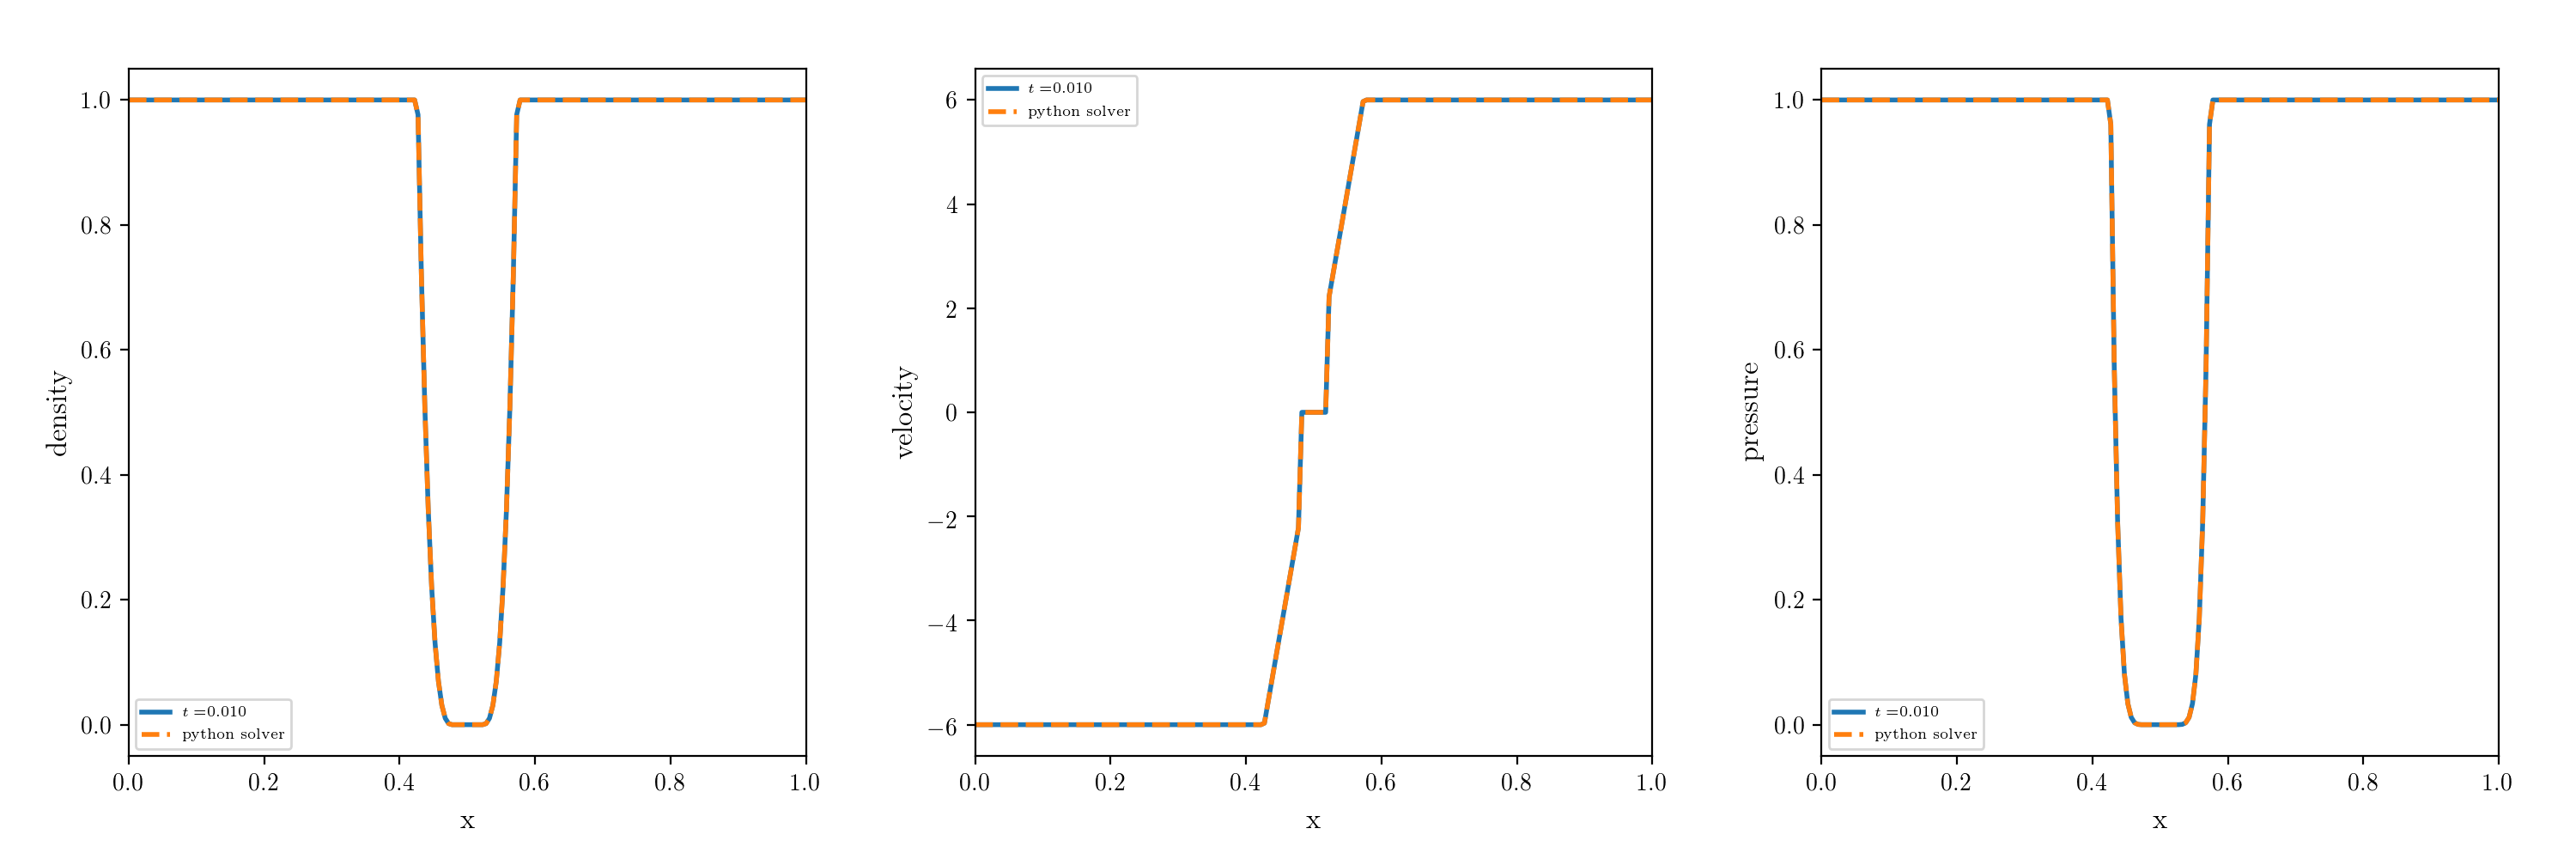
\includegraphics[width=.9\textwidth]{./figures/riemann-vacuum-generating-RIEMANN-EXACT-overplotted.png}%
	\caption{Exact solver for vacuum generating conditions. Expected result.}
	\includegraphics[width=.9\textwidth]{../riemann-vacuum-generating-RIEMANN-EXACT-overplotted.png}%
	\caption{Exact solver for vacuum generating conditions. Obtained result.}
\end{figure}






\end{document}
